\documentclass[10pt,a4paper]{article}
\usepackage[utf8]{inputenc}
\usepackage{amsmath}
\usepackage{amsfonts}
\usepackage{amssymb}
\usepackage{pdfpages}
\author{Elvis Nava 870234 - Dario Ostuni 870321}
\title{Manuale Utente\\
 Progetto Basi di Dati\\
\textit{DungeonAsDB - Comelico Simulator 2017}}
\date{Gennaio 2017}

\usepackage{graphicx}
\graphicspath{ {img_manuale/} }

\usepackage{listings}
\usepackage{color}

\definecolor{dkgreen}{rgb}{0,0.6,0}
\definecolor{gray}{rgb}{0.5,0.5,0.5}
\definecolor{mauve}{rgb}{0.58,0,0.82}

\lstset{frame=tb,
  language=bash,
  aboveskip=3mm,
  belowskip=3mm,
  showstringspaces=false,
  columns=flexible,
  basicstyle={\small\ttfamily},
  numbers=none,
  numberstyle=\tiny\color{gray},
  keywordstyle=\color{blue},
  commentstyle=\color{dkgreen},
  stringstyle=\color{mauve},
  breaklines=true,
  breakatwhitespace=true,
  tabsize=3
}

\begin{document}

\maketitle

\section{Installazione dell'applicazione}
Per l'installazione dell'applicazione è richiesta la presenza dei seguenti pacchetti software:
\begin{itemize}
\item apache 2.4+
\item python 3.4+
\item psycopg2 2.6+
\item PostgreSQL 9.4+
\item PL/Python 3+
\end{itemize}

\subsection{Confugirazione Database}
Prima di importare gli script SQL occorre creare un database \texttt{game} e un utente \texttt{game} proprietario di tale database. Se non si ha intenzione di modificare i sorgenti dell'applicazione web, usare come password \texttt{comsimgame17}, altrimenti bisognerà sostituire il secondo parametro della funzione a riga 23 di \texttt{index.py}.

Mentre si è loggati come \texttt{game}, importare i file \texttt{gameschema.sql} e \texttt{content.sql} nell'ordine specificato per creare le relazioni e popolare il database con i dati di gioco iniziali. Occorre invece essere loggati come \texttt{postgres} per l'importazione successiva di \texttt{functions.sql} e \texttt{triggers.sql}, siccome il linguaggio procedurale utilizzato, \texttt{plpython3u}, è untrusted.

\subsection{Configurazione Applicazione Web}
Occorre spostare il contenuto della cartella \texttt{site} in una cartella a piacimento, a condizione che tutte le cartelle del percorso all'insù dalla cartella scelta verso \texttt{/} abbiano i bit di lettura e di eseguibilità attivati.

Occorre in seguito modificare il file di configurazione di apache aggiungendo in fondo:

\begin{lstlisting}
Alias /game "cartellascelta"
<Directory "cartellascelta">
    DirectoryIndex index.py
    Options +ExecCGI +FollowSymlinks
    AddHandler cgi-script .py
    AllowOverride None
    Require all granted
</Directory>
\end{lstlisting}

Se non è già abilitato, occorre abilitare mod\_cgi su apache.

\section{Istruzioni di gioco}
Per iniziare a giocare connettersi con il browser alla pagina di gioco hostata in locale. Una versione online si può trovare su https://eip.ovh/game

\subsection{Registrazione e Login}
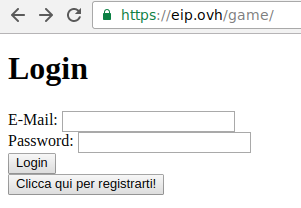
\includegraphics[scale=0.7]{1login}\\
Se si possiede già un account, effettuare il login inserendo i propri dati, altrimenti cliccare sul pulsante per registrarsi.\\
\\
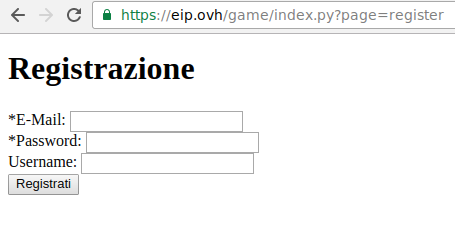
\includegraphics[scale=0.7]{2registrazione}\\
Nella schermata di registrazione occorre inserire un'E-Mail formattata correttamente, una password, e opzionalmente un nome utente.

\subsection{Creazione e selezione del personaggio}
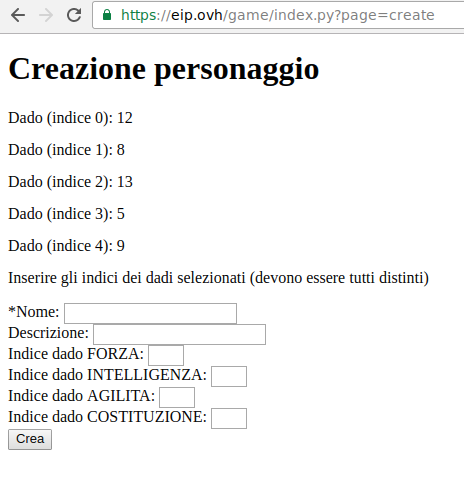
\includegraphics[scale=0.7]{3creazionepersonaggio}\\
Dopo il primo login si verrà trasferiti alla pagina di creazione del personaggio. Vengono effettuati 5 lanci di dadi 3d6 e i risultati sono mostrati sulla pagina. Occorre inserire il nome del personaggio, una descrizione opzionale, e scegliere per ogni attributo base di gioco l'indice (0-4) del dado scelto. Non è possibile scegliere più volte lo stesso dado.\\
\\
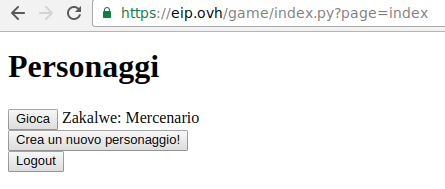
\includegraphics[scale=0.7]{4selezionepersonaggio}\\
Una volta creato il primo personaggio occorrerà selezionarlo per giocare. Da questa schermata di selezione è possibile creare altri personaggi e iniziare o riprendere le partite con qualunque personaggio ancora in vita.

\subsection{Schermata di gioco principale}
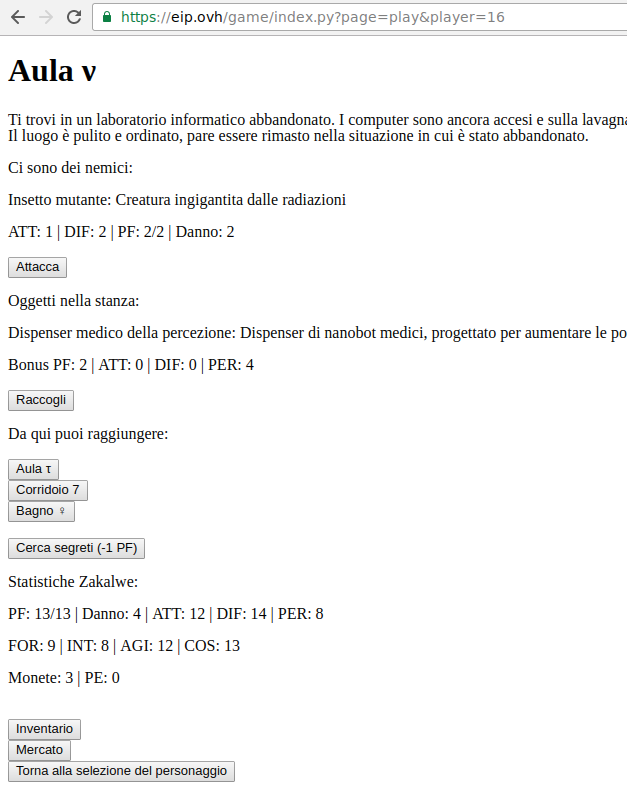
\includegraphics[scale=0.6]{5schermatadigioco}\\
La schermata di gioco principale presenta una serie di informazioni:
\begin{itemize}
\item Descrizione della stanza in cui si trova il personaggio.
\item Elenco di nemici presenti con la possibilità di attaccarli.
\item Elenco di oggetti a terra con la possibilità di raccoglierli.
\item Elenco delle stanze adiacenti con la possibilità di raggiungerle.
\item Pulsante per cercare passaggi segreti o oggetti nascosti (Consuma 1 PF!).
\item Statistiche del personaggio tra cui i Punti Ferita rimanenti, gli attributi di gioco, le monete raccolte e i Punti Esperienza.
\item Pulsanti per raggiungere le schermate dell'Inventario e del Mercato di gioco.
\item Pulsante per uscire dalla partita e tornare alla schermata di selezione del personaggio.
\end{itemize}
Attenzione: i nemici attaccheranno il personaggio quando questo sceglierà di attaccare, raccogliere oggetti, andarsene in un'altra stanza o cercare segreti!

\subsection{Inventario}
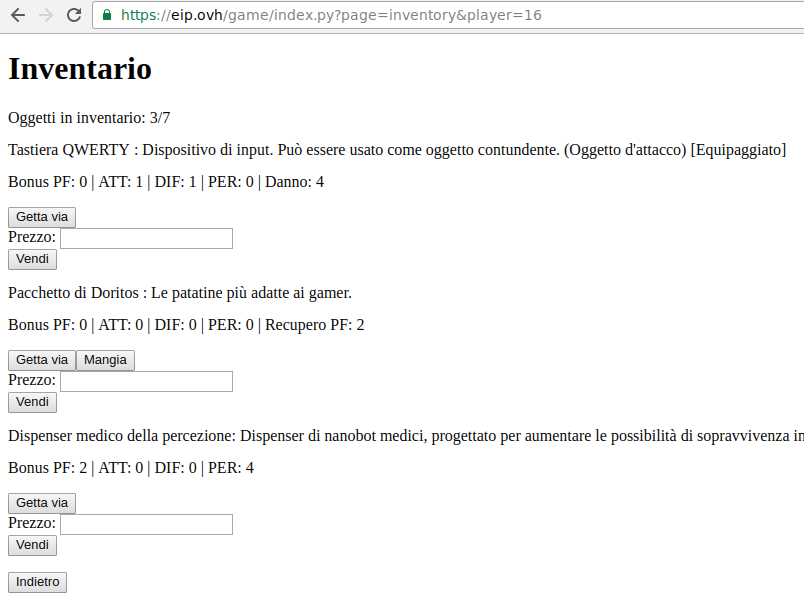
\includegraphics[scale=0.5]{6inventario}\\
La schermata dell'inventario permette di visualizzare gli oggetti di cui il personaggio è in possesso ed effettuare alcune azioni con essi, in particolare:
\begin{itemize}
\item Gettare a terra oggetti non desiderati.
\item Equipaggiare oggetti di attacco o di difesa Può essere equipaggiato solo un oggetto per tipo alla volta. Se si equipaggia un nuovo oggetto sarà rimosso al precedente lo status di [Equipaggiato].
\item Mangiare oggetti di tipo "cibo".
\item Consumare oggetti di tipo "consumabile". I bonus di tali oggetti vengono applicati solo dopo il consumo e scadono quando il personaggio si sposta da una stanza all'altra.
\item Mettere in vendita oggetti sul mercato, specificando il prezzo in monete.
\end{itemize}

\subsection{Mercato di gioco}
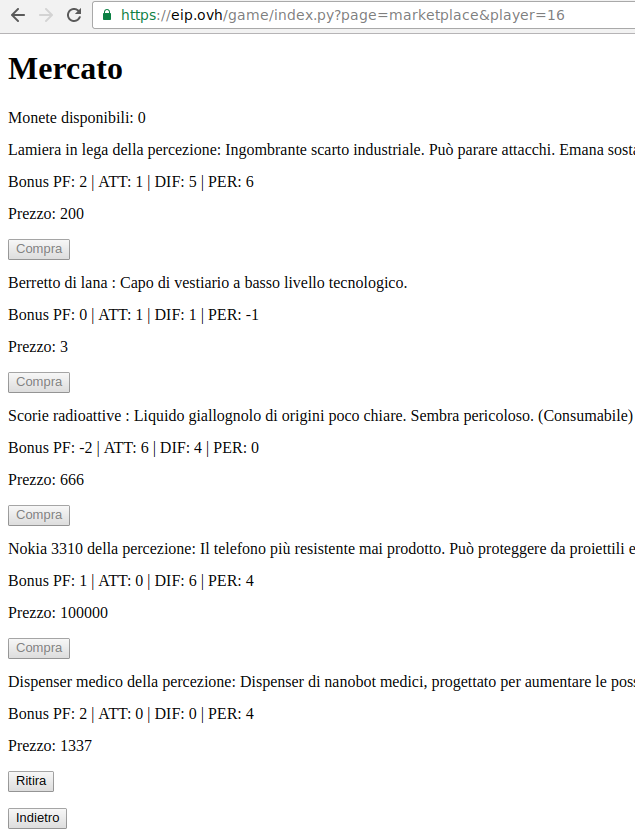
\includegraphics[scale=0.5]{7mercato}\\
La schermata del mercato di gioco mostra l'elenco degli oggetti messi in vendita da ogni utente dell'applicazione. Se il personaggio dispone di monete sufficienti può comprare un oggetto, che sarà trasferito nel suo inventario. È inoltre possibile ritirare dalla vendita i propri oggetti.

\end{document}